\section{What are your favorite memories of each of your children growing up?}
I enjoy spending time with my children They each have a keen mind and a great sense of humor.

Timothy- first born, absorbing observer of what is around him, articulate, values people and engages with and listens to them
From an early age Tim has worked at communicating ideas to people.
He has become quite an articulate and skilled communicator.
Even at an early age before he had the vocabulary to speak his ideas he was able to communicate.
One evening John and I were sitting at the dining table when Tim headed back the hallway toward his room.
He was not gone long.
He came back into the kitchen pointing back toward the bedroom with one hand, while opening and closing the other and blinking his eyes open and closed.
No words were needed we knew immediately that he wanted us to come back and turn on the light in his bedroom.
\begin{figure}
\centering
\includegraphics[width=0.9\textwidth]{our_family/6.jpg}
\caption{
"Amanda, you've got wax in your ear"
}
\end{figure}

\begin{figure}
\centering
\includegraphics[width=0.9\textwidth]{our_family/7.jpg}
\caption{
"Right back at you Timothy, so do you"
}
\end{figure}

\begin{figure}
\centering
\includegraphics[width=0.9\textwidth]{our_family/8.jpg}
\caption{
Here is Tim telling one of his first jokes.
}
\end{figure}

\begin{figure}
\centering
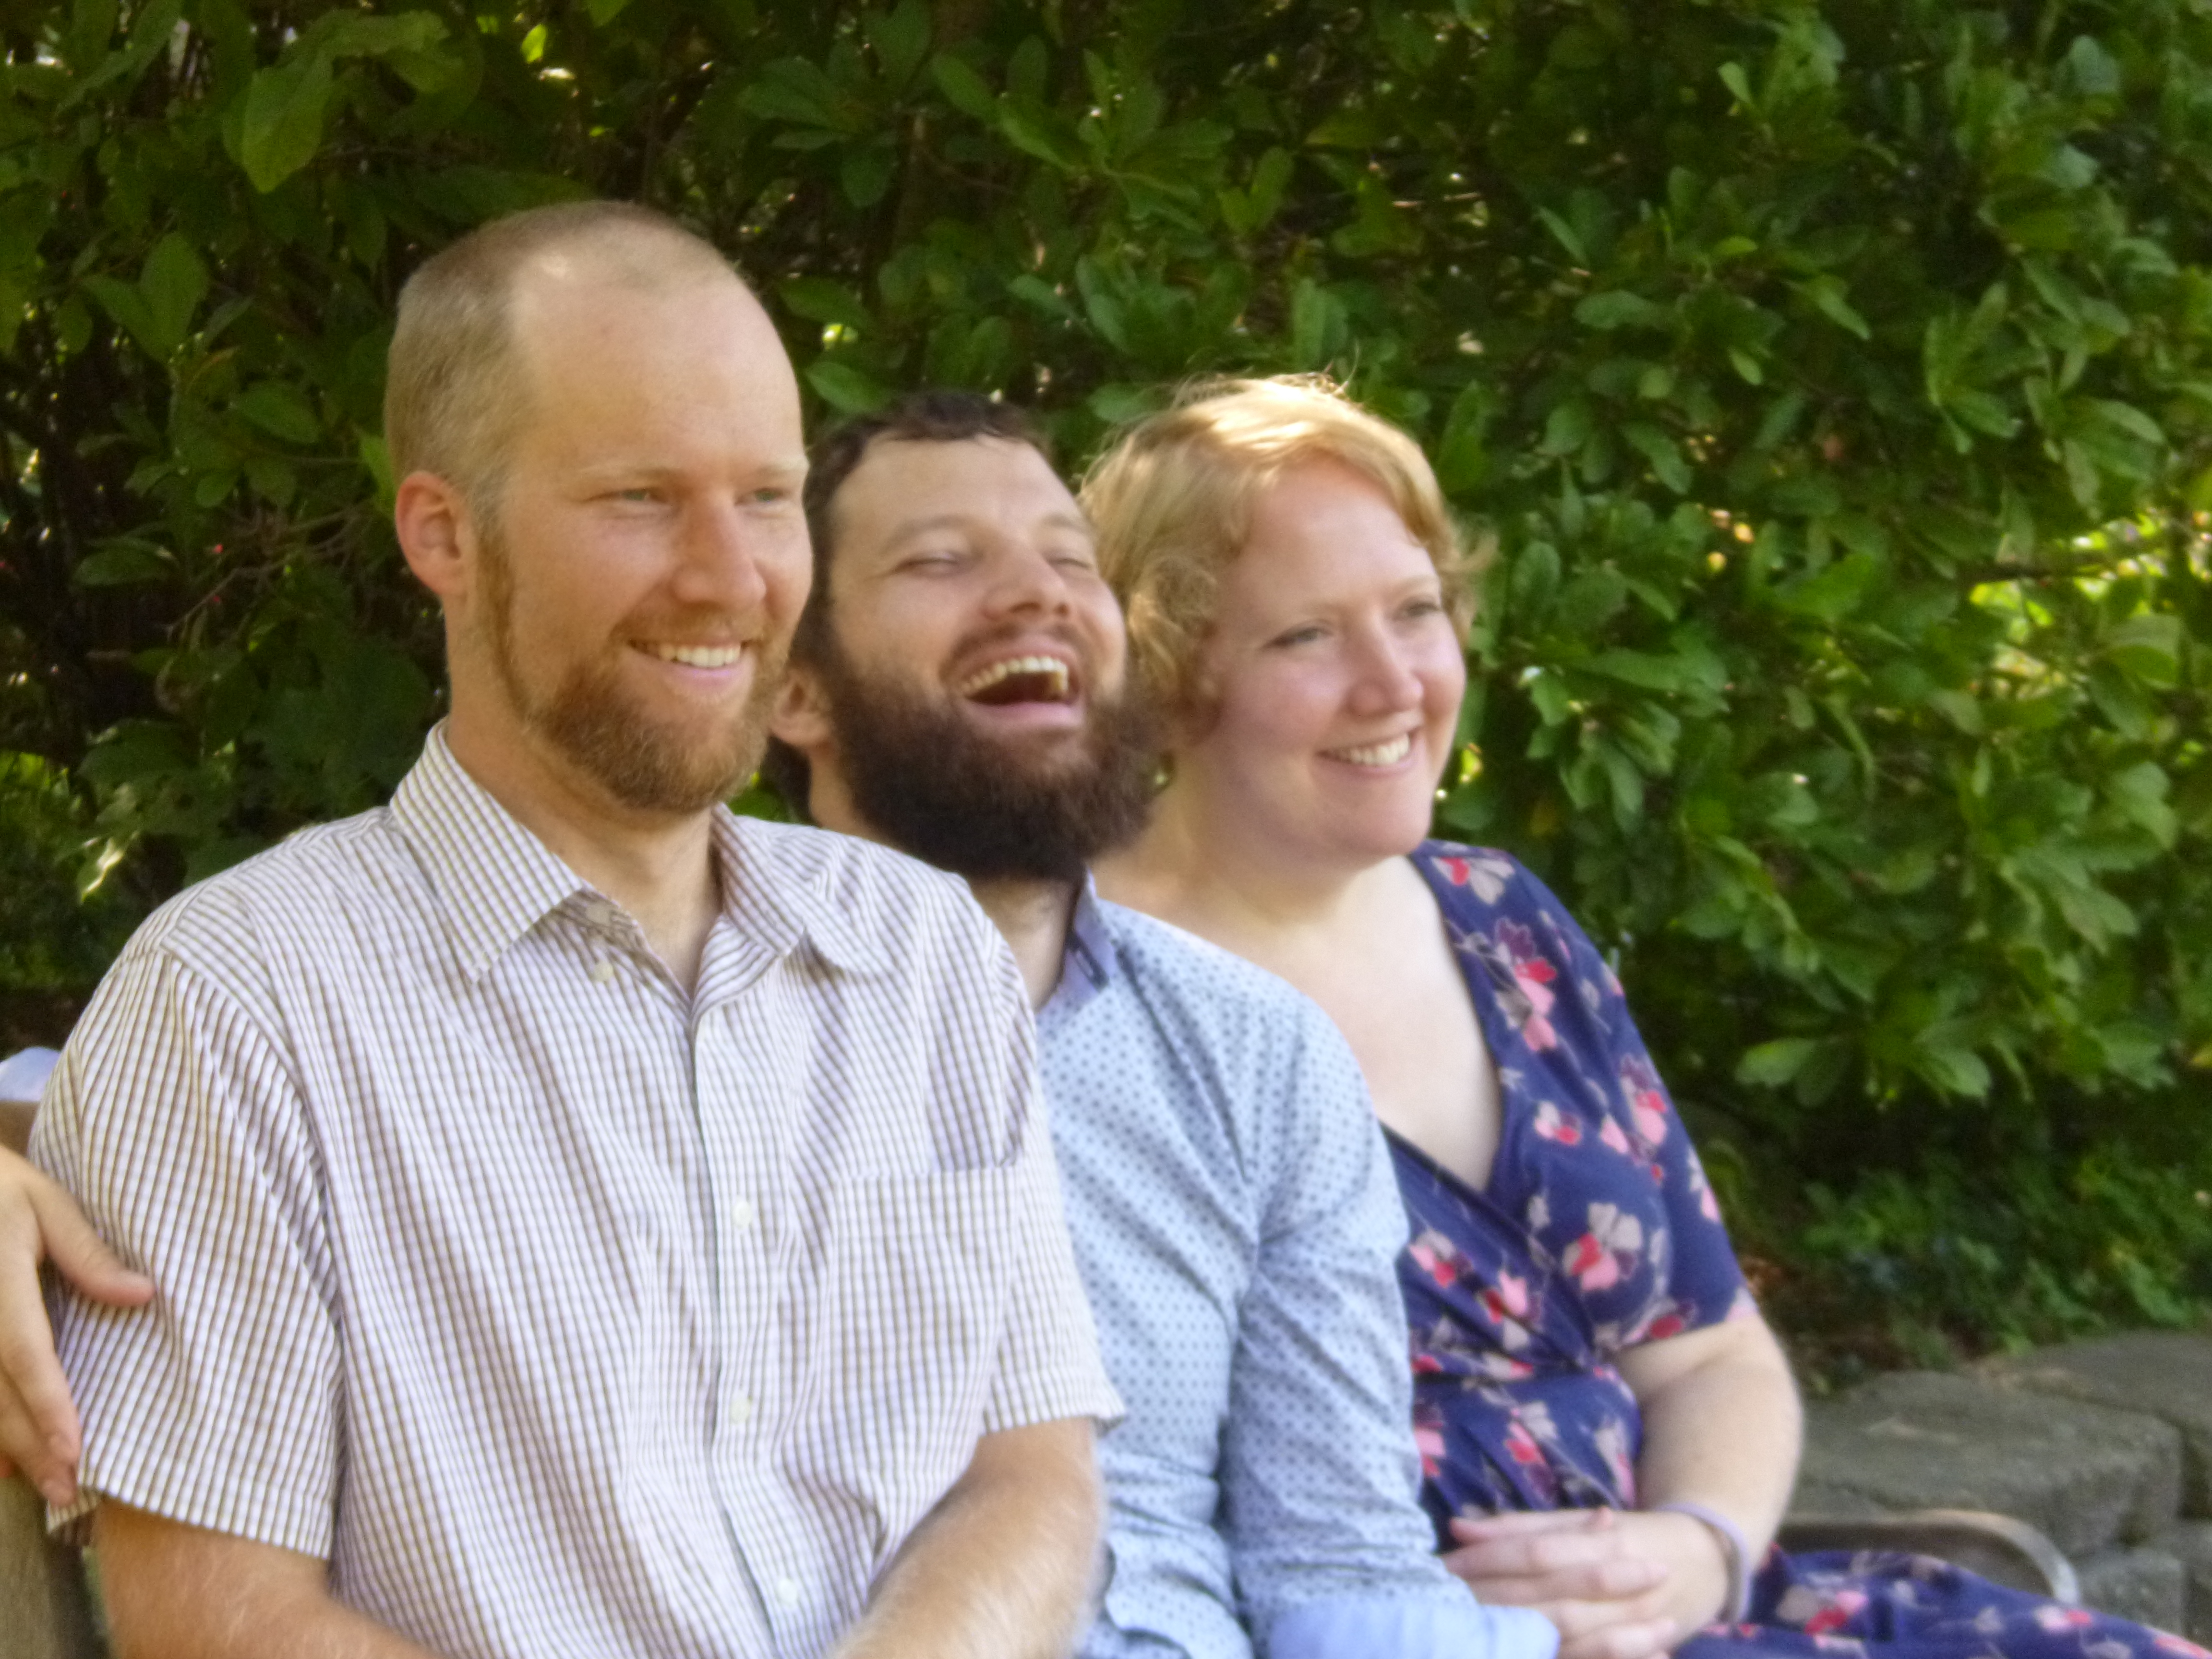
\includegraphics[width=0.9\textwidth]{our_family/9.jpg}
\caption{
And now for the punch line.
}
\end{figure}


Abigail- only daughter, brings energy into the room, able to give a significant critic, compassionate, loyal, aware of others thoughts and feelings
Sometimes Abigail likes to organize people.
One Sunday after church she asked if her cousin Laura could spend the afternoon with her.
For whatever reason both her parents and Laura's parents said no to that plan.
The Jackson van left for home and John and I finished up whatever it was that we were doing and then looked for Abigail and Jonathan.
Tim was with us but we could not find Abigail and Jonathan.
The church is not very large so we soon knew that the two children were not there.
This was before the days of cell phones, but there was a phone in the church.
We soon learned that when the Jackson pulled into their garage at home they found two little stowaways behind the back seat of the van.
I'm guessing that Abigail was the mastermind who planned the escapade and Jonathan went along with the idea.
I suppose Laura and Ben were looking forward to having two cousins to play with for the afternoon.
Needless to say we had a longer trip home from church that day since we first drove to the Jackson house to pick up our two missing children.
\begin{figure}
\centering
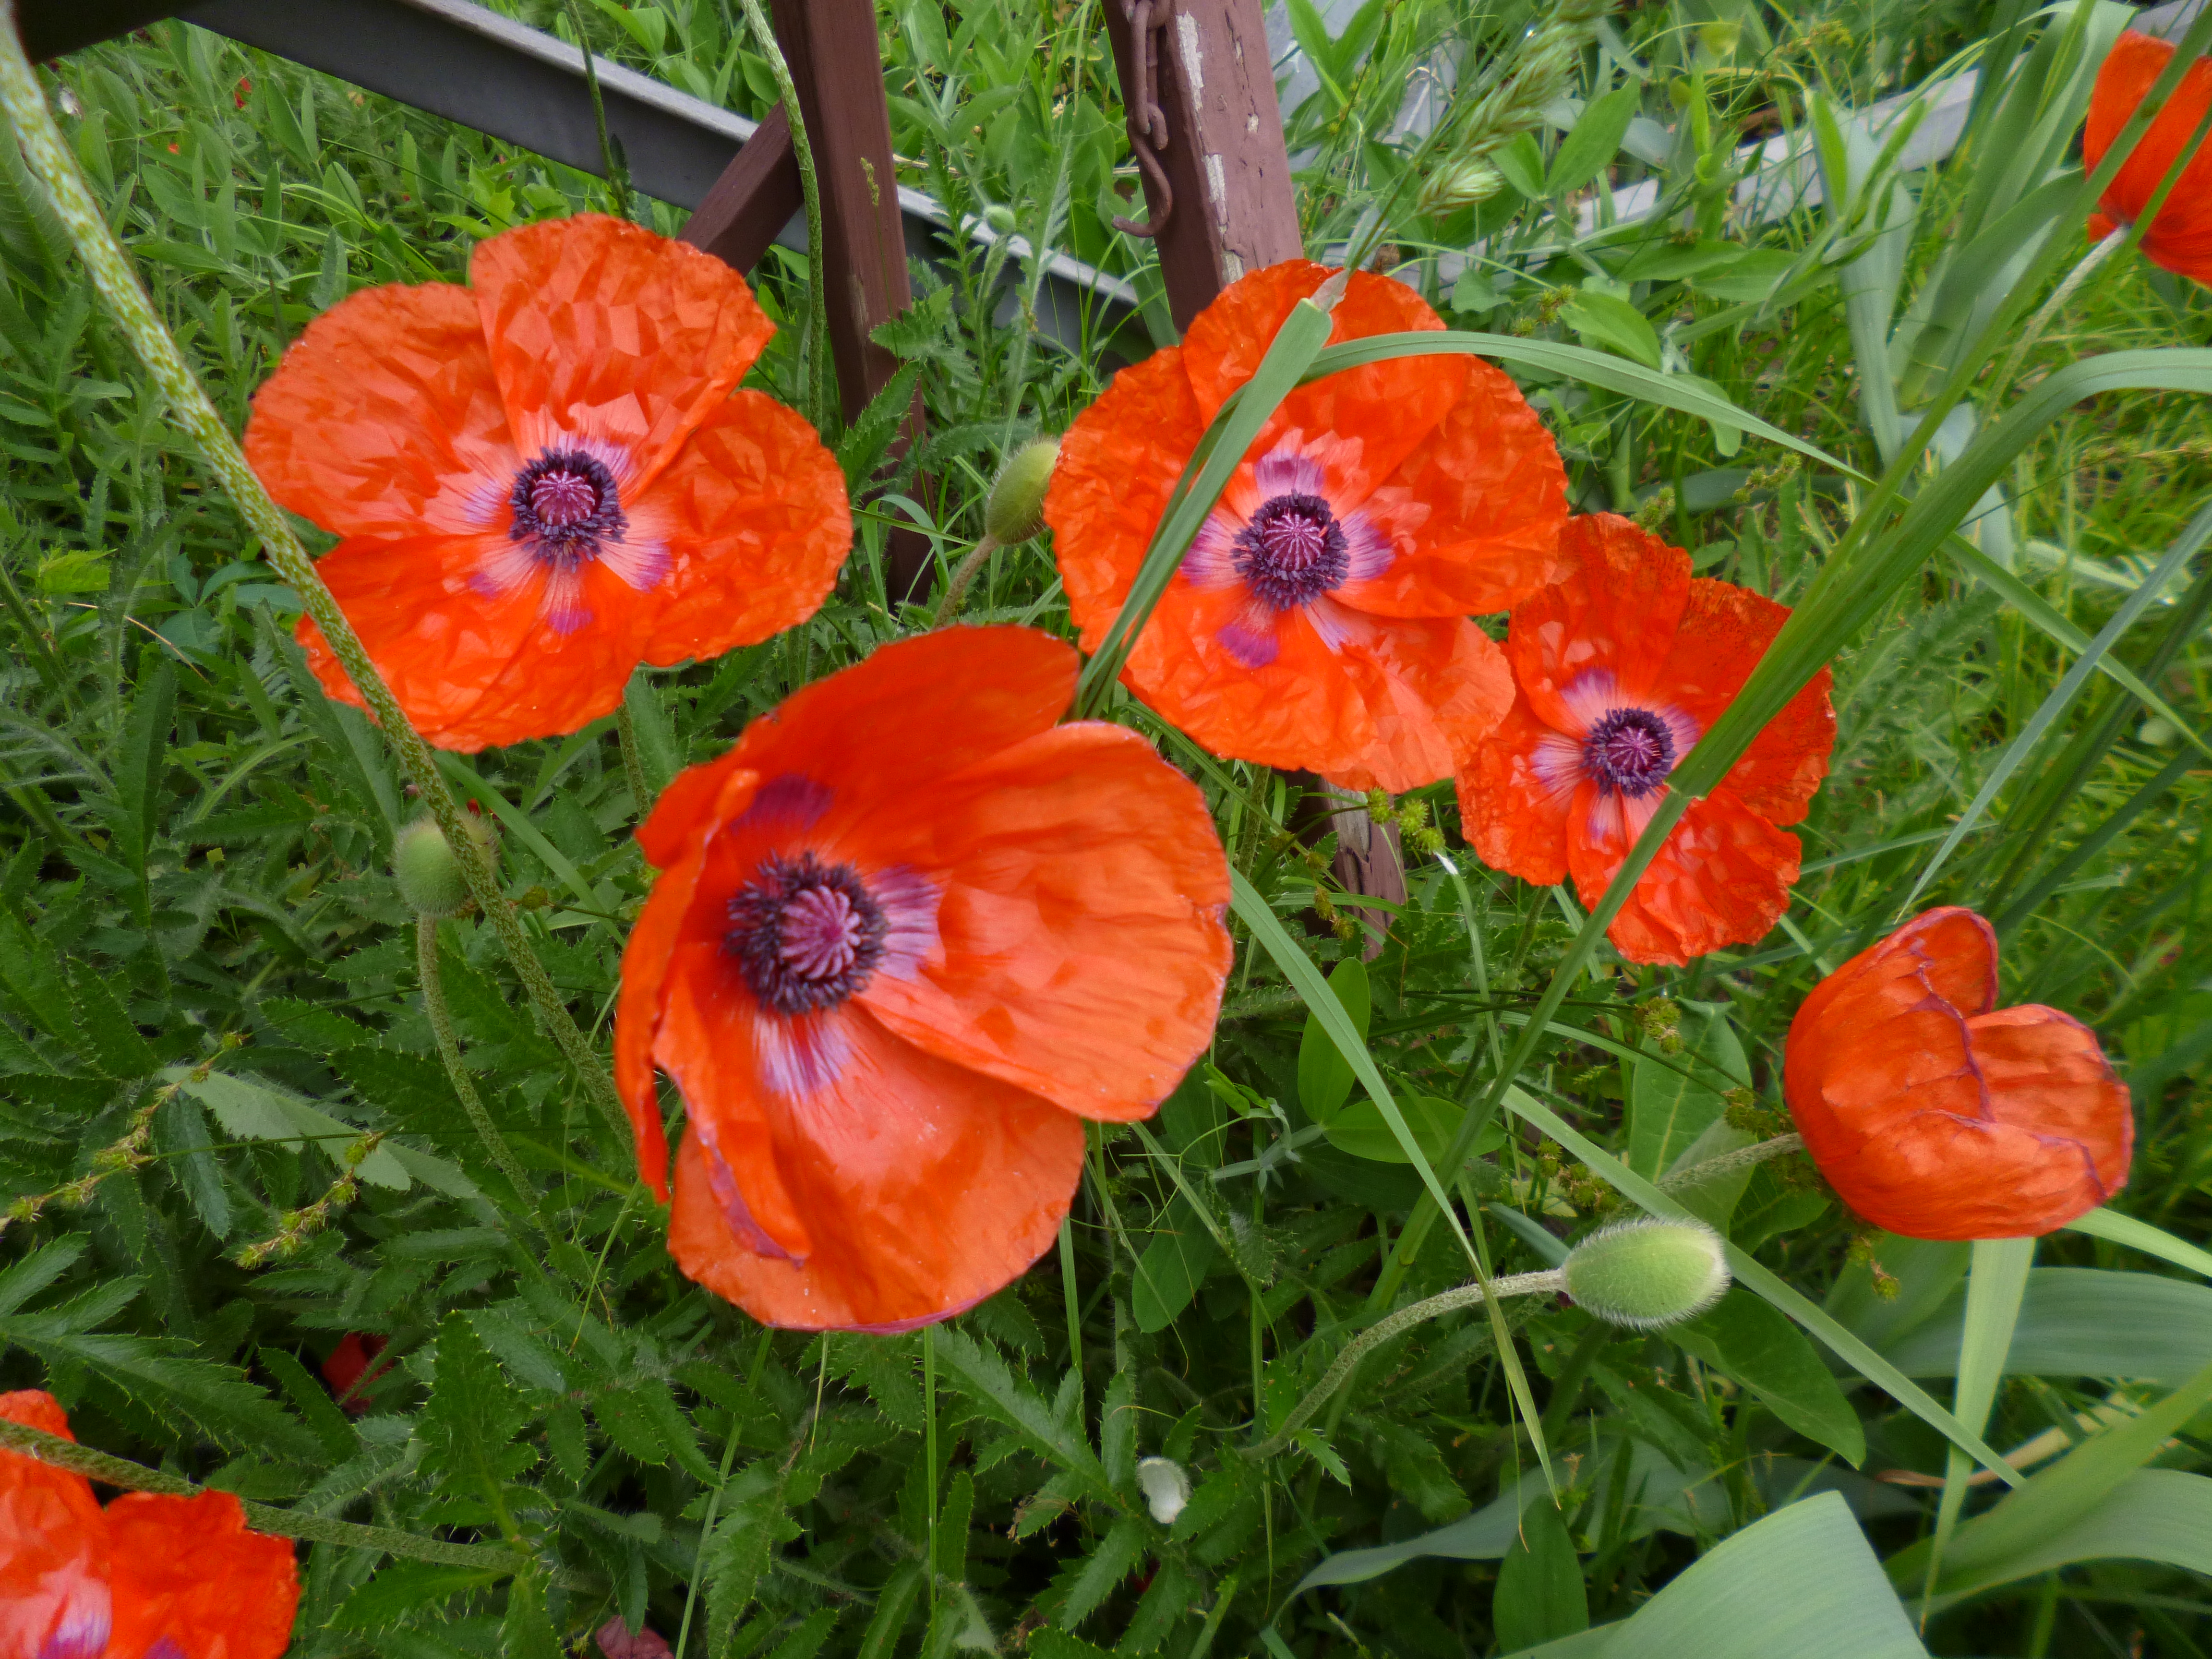
\includegraphics[width=0.9\textwidth]{our_family/10.jpg}
\caption{
Queen of the wash basket
}
\end{figure}

\begin{figure}
\centering
\includegraphics[width=0.9\textwidth]{our_family/11.jpg}
\caption{
Don't worry I've got things under control
}
\end{figure}

\begin{figure}
\centering
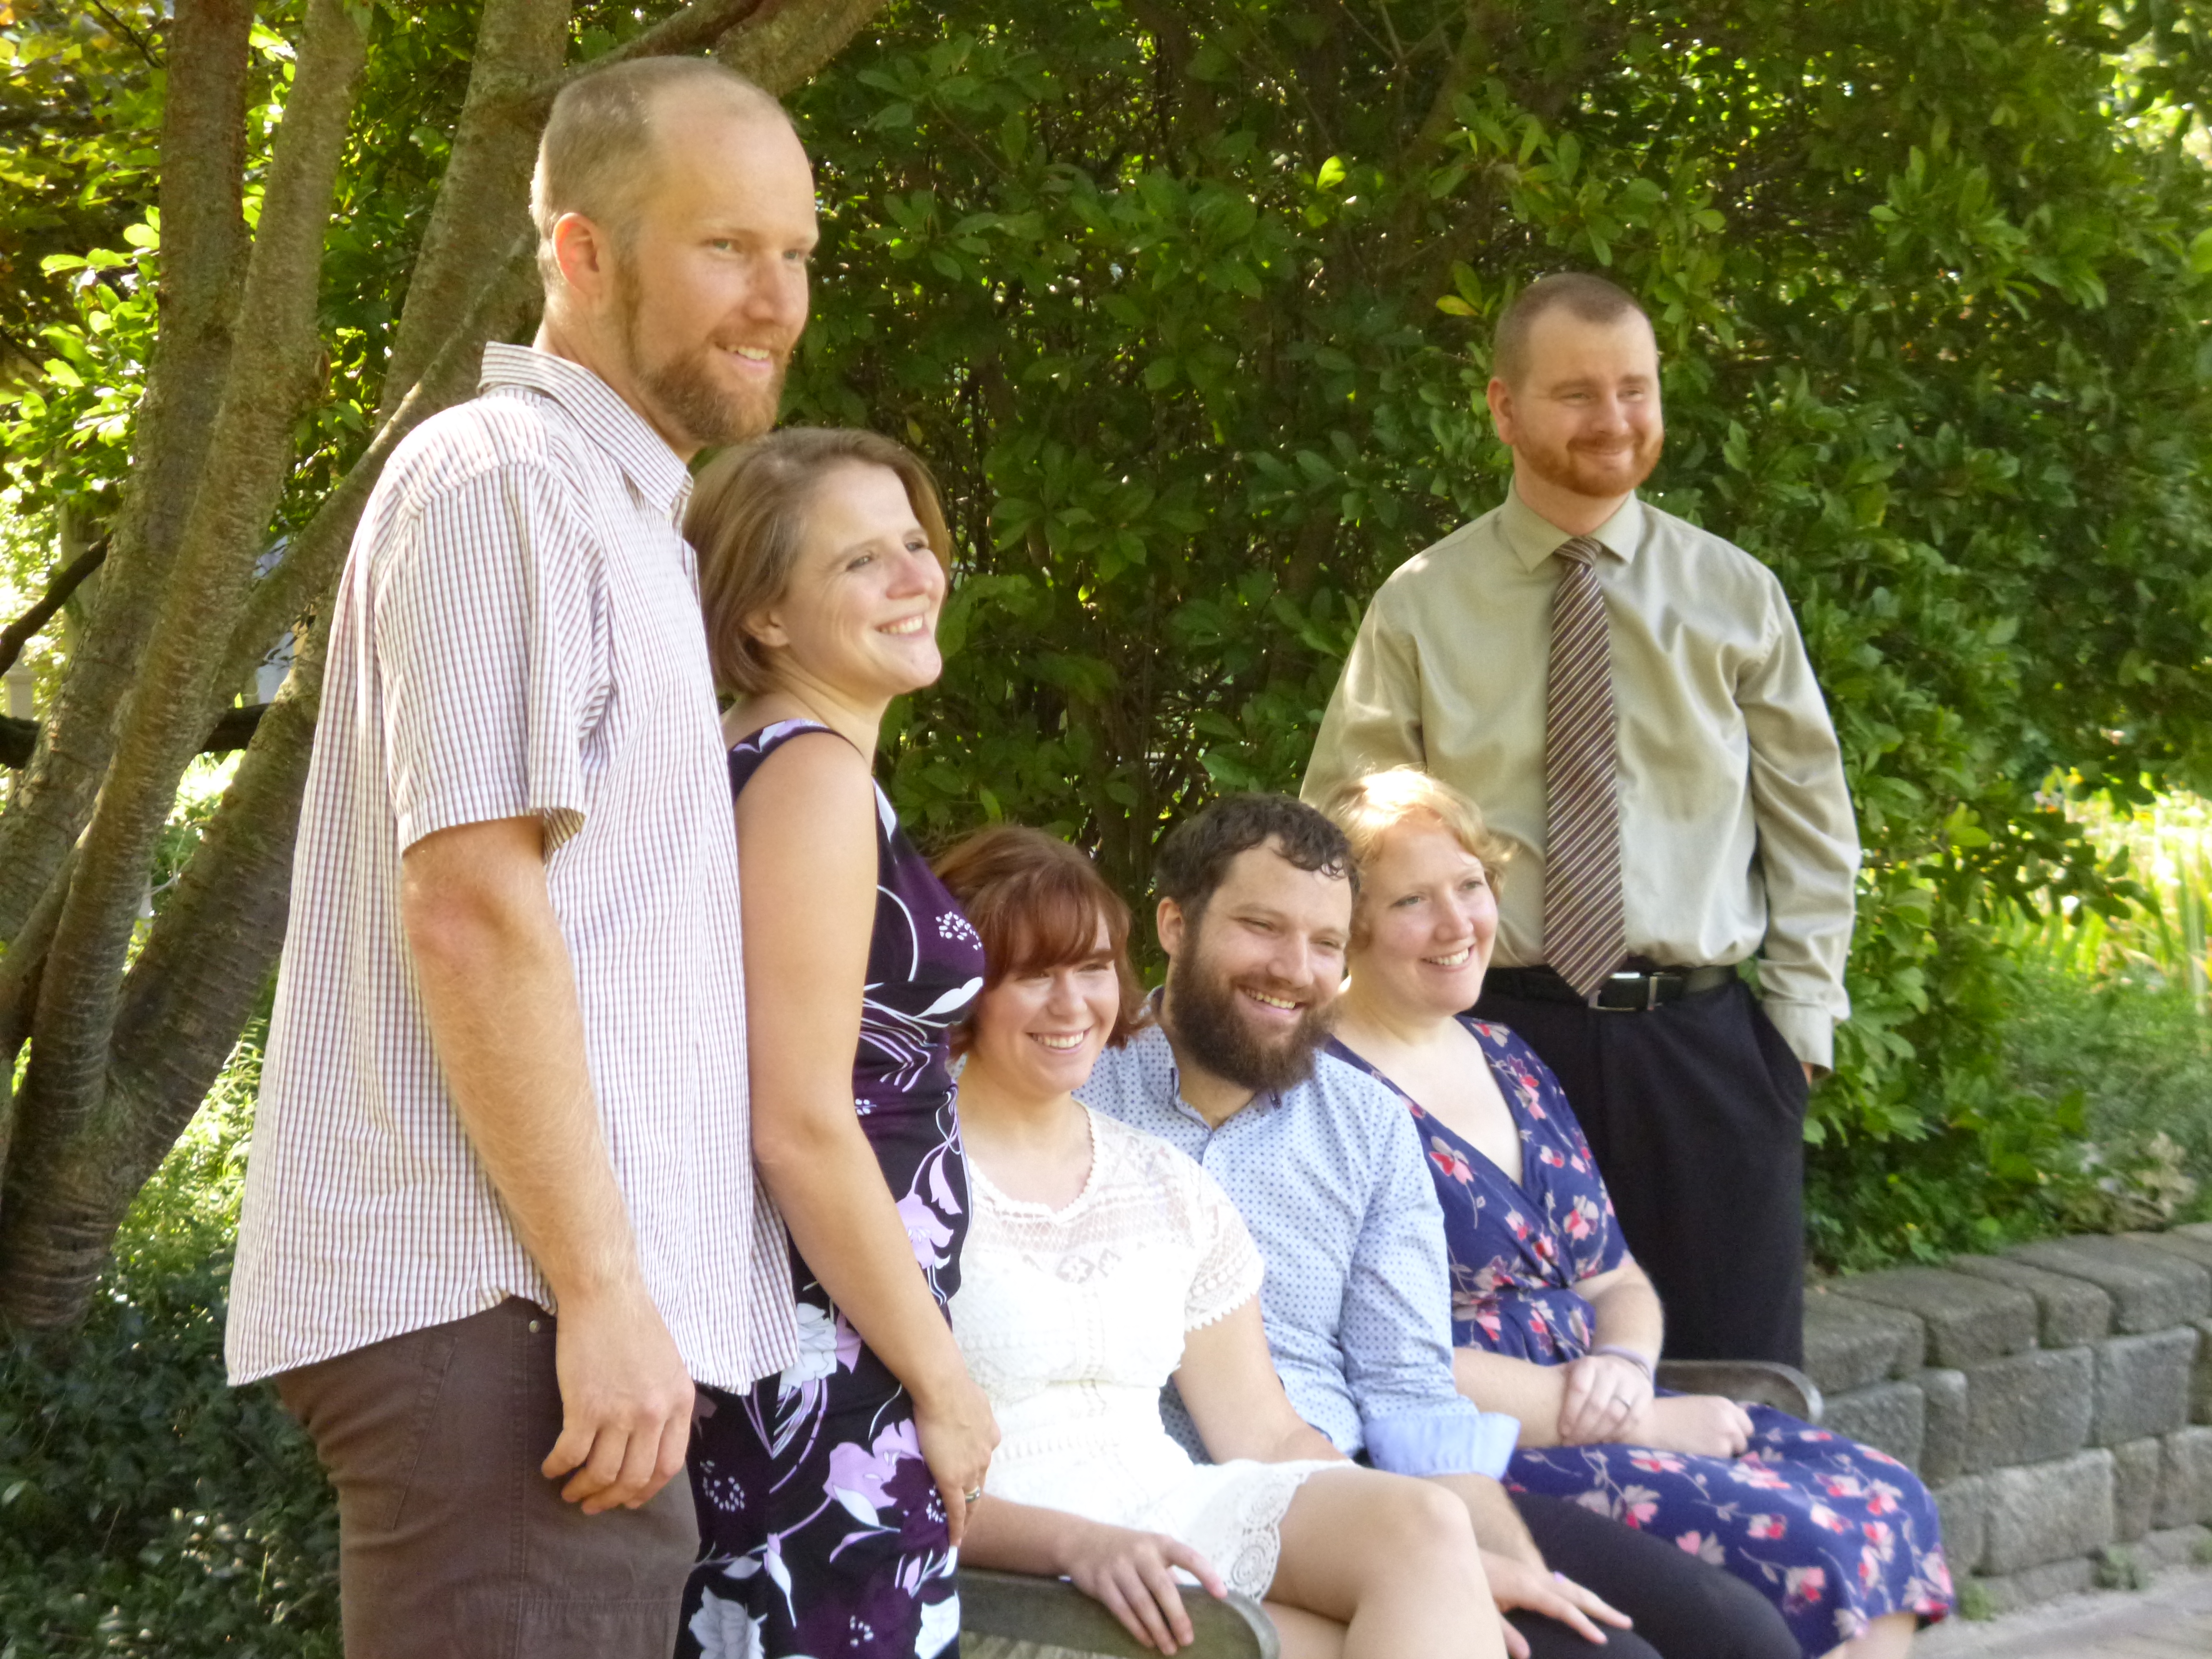
\includegraphics[width=0.9\textwidth]{our_family/12.jpg}
\caption{
Little Champ of the...
}
\end{figure}

\begin{figure}
\centering
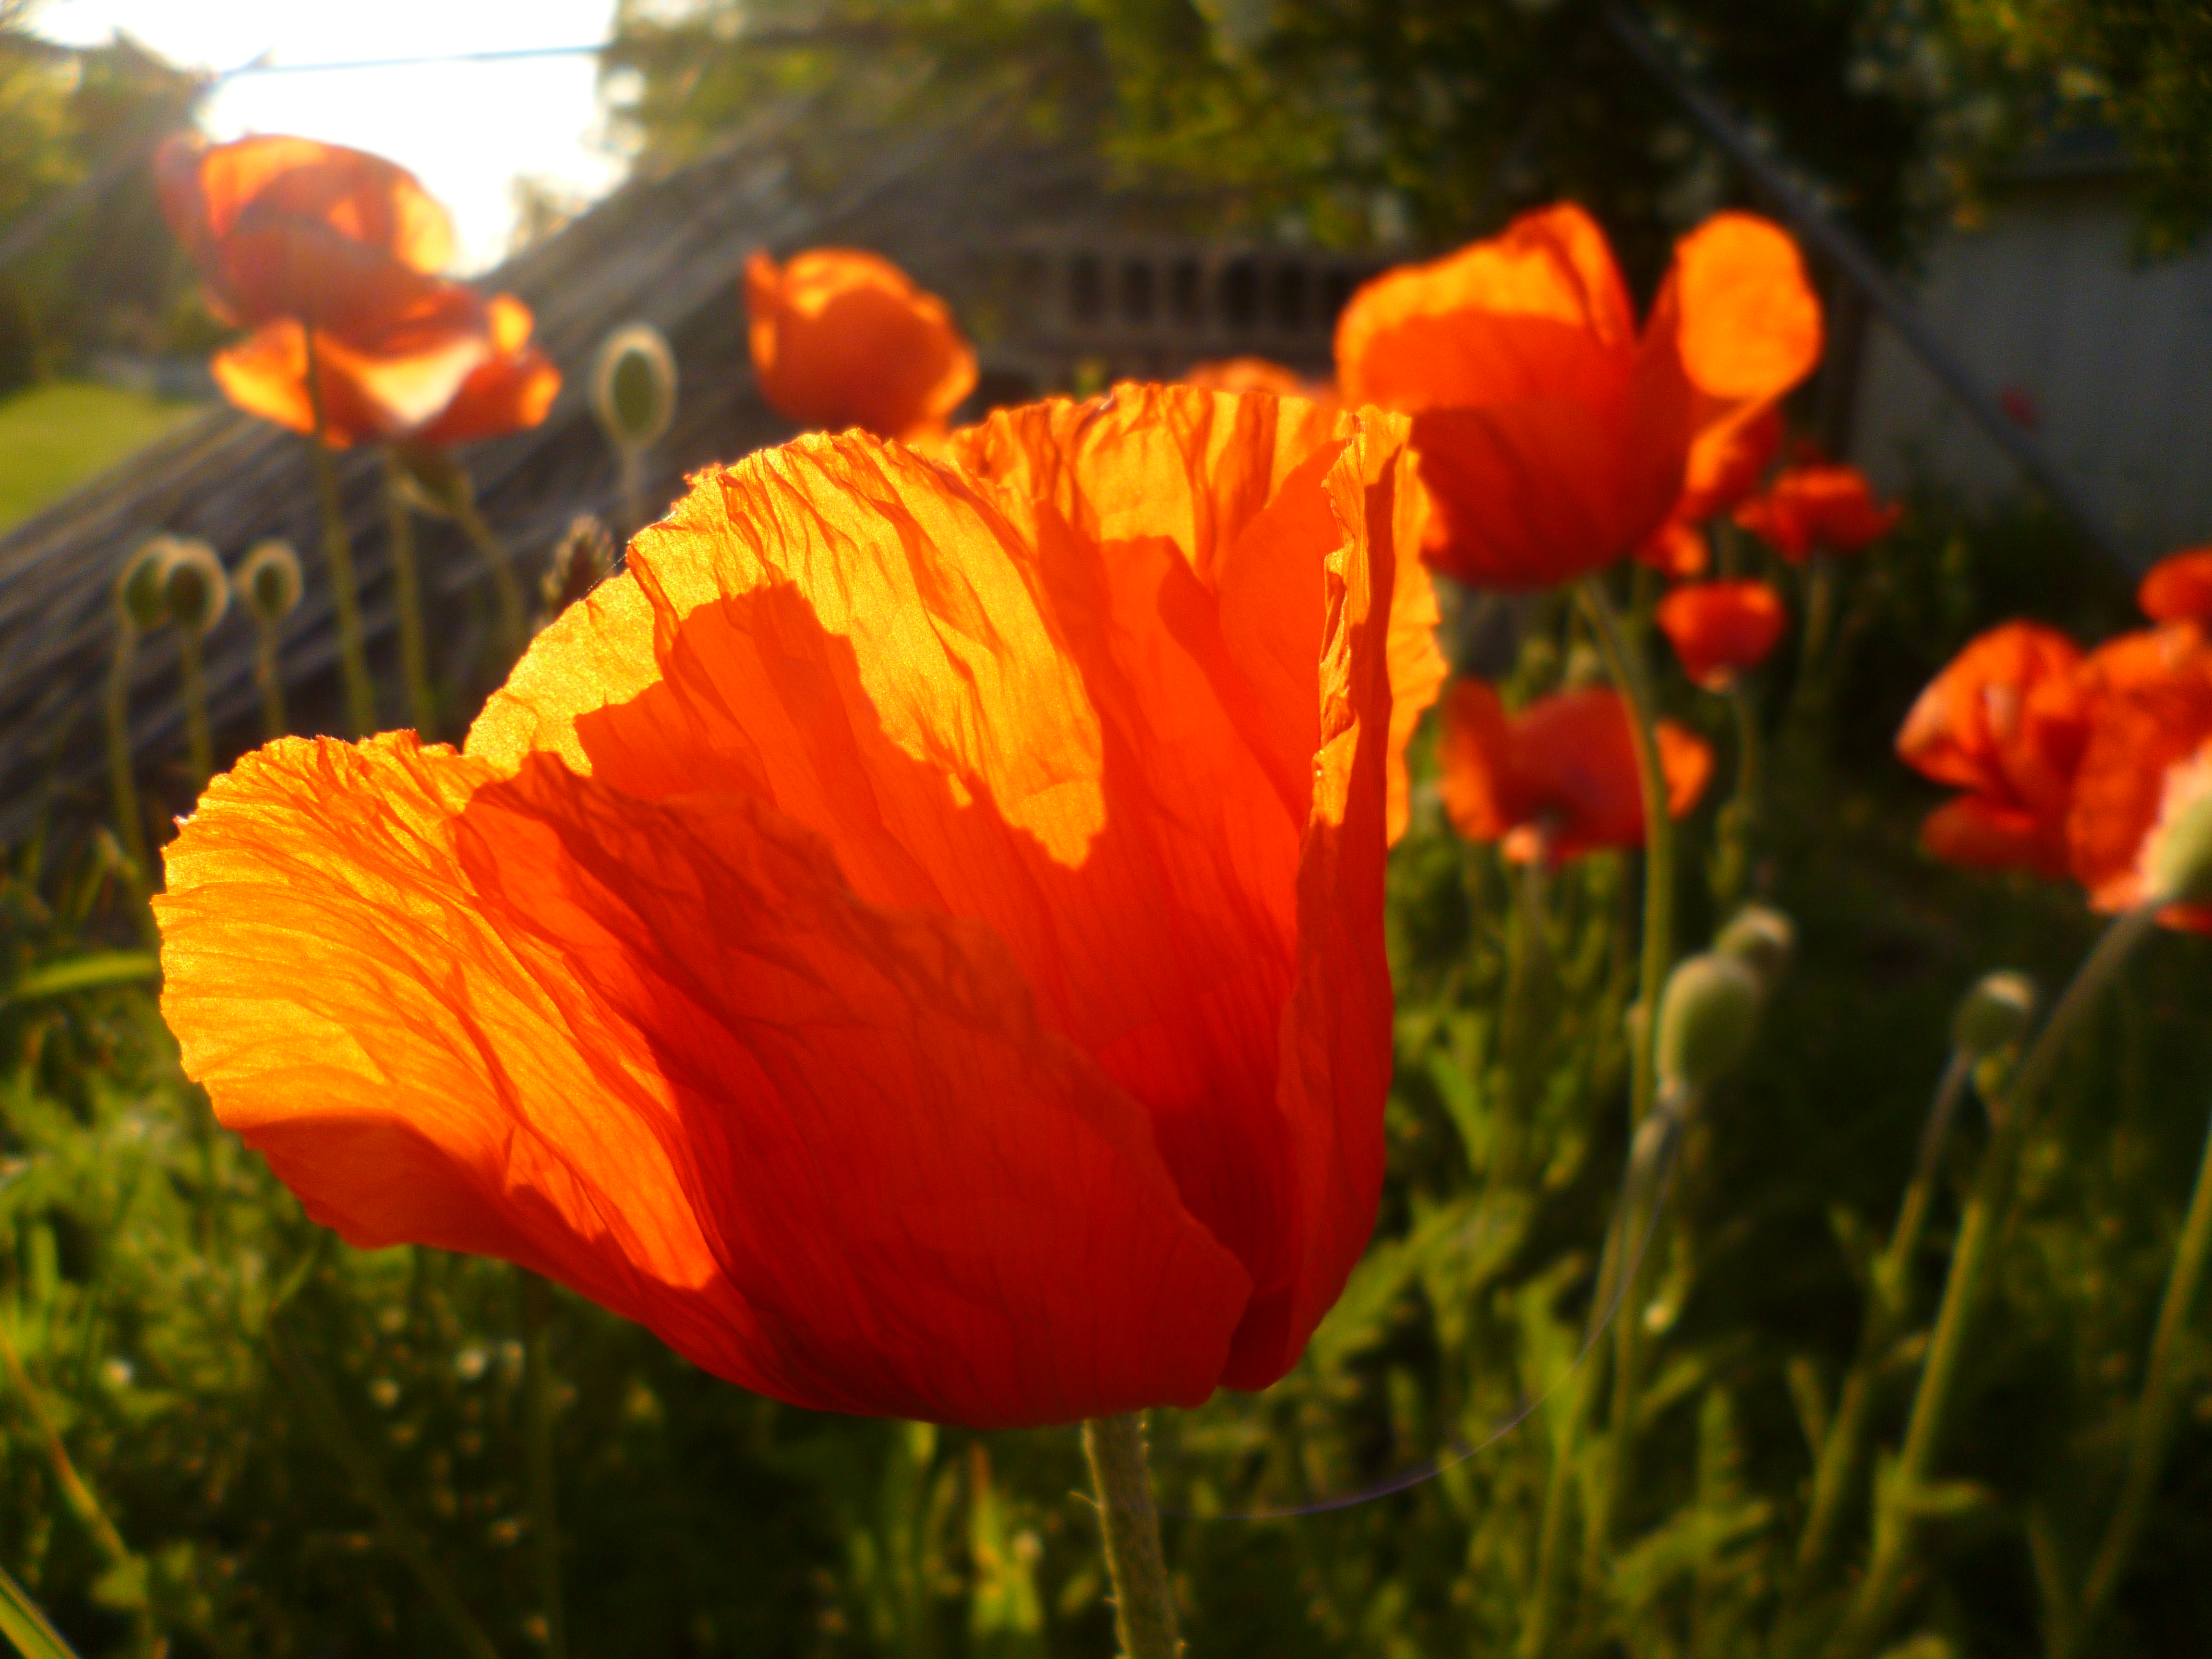
\includegraphics[width=0.9\textwidth]{our_family/13.jpg}
\caption{
Staring contest.
}
\end{figure}

Jonathan- the youngest, ability to analyze and make wise observations, brain power, make important connections, sensitive to others
From an early age Jonathan was exploring his world. 
\begin{figure}
\centering
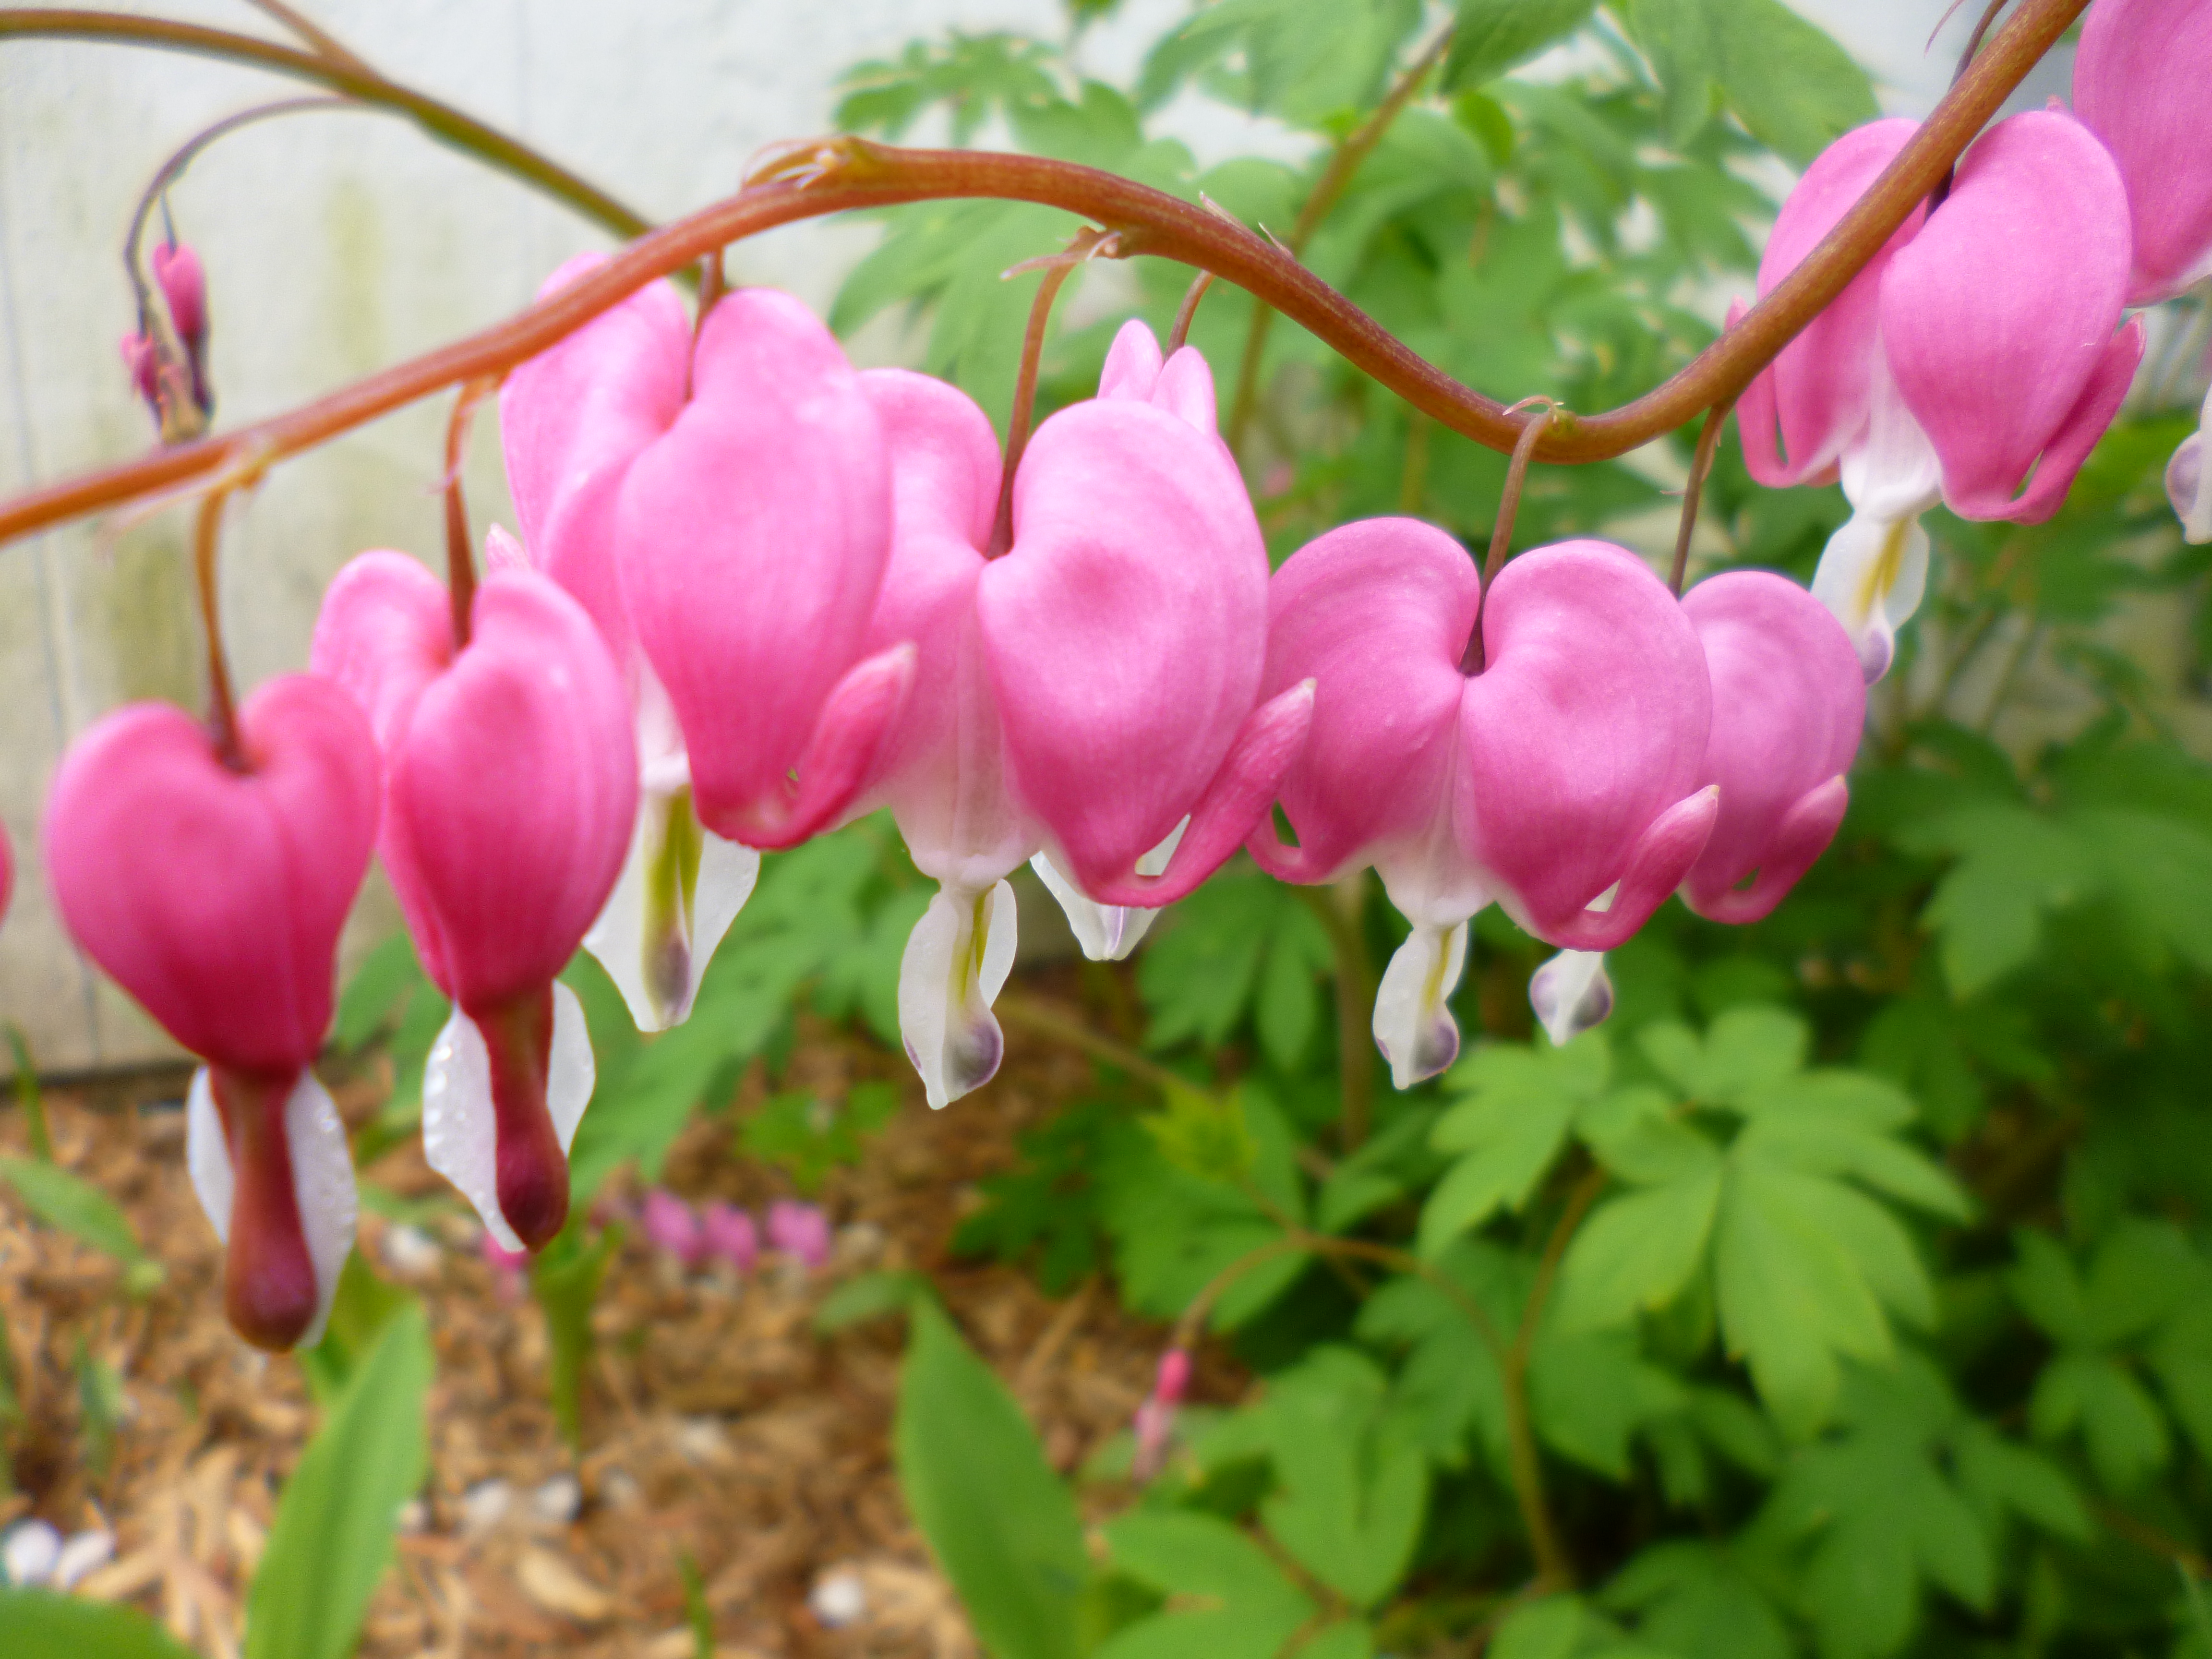
\includegraphics[width=0.9\textwidth]{our_family/14.jpg}
\caption{
"Well folks, I find this to be gritty and cold." 
}
\end{figure}
He had two older siblings vying for his attention.
\begin{figure}
\centering
\includegraphics[width=0.9\textwidth]{our_family/15.jpg}
\caption{
"What is it like to be a fish"
}
\end{figure}
This may have freed him to forge his own path. 
\begin{figure}
\centering
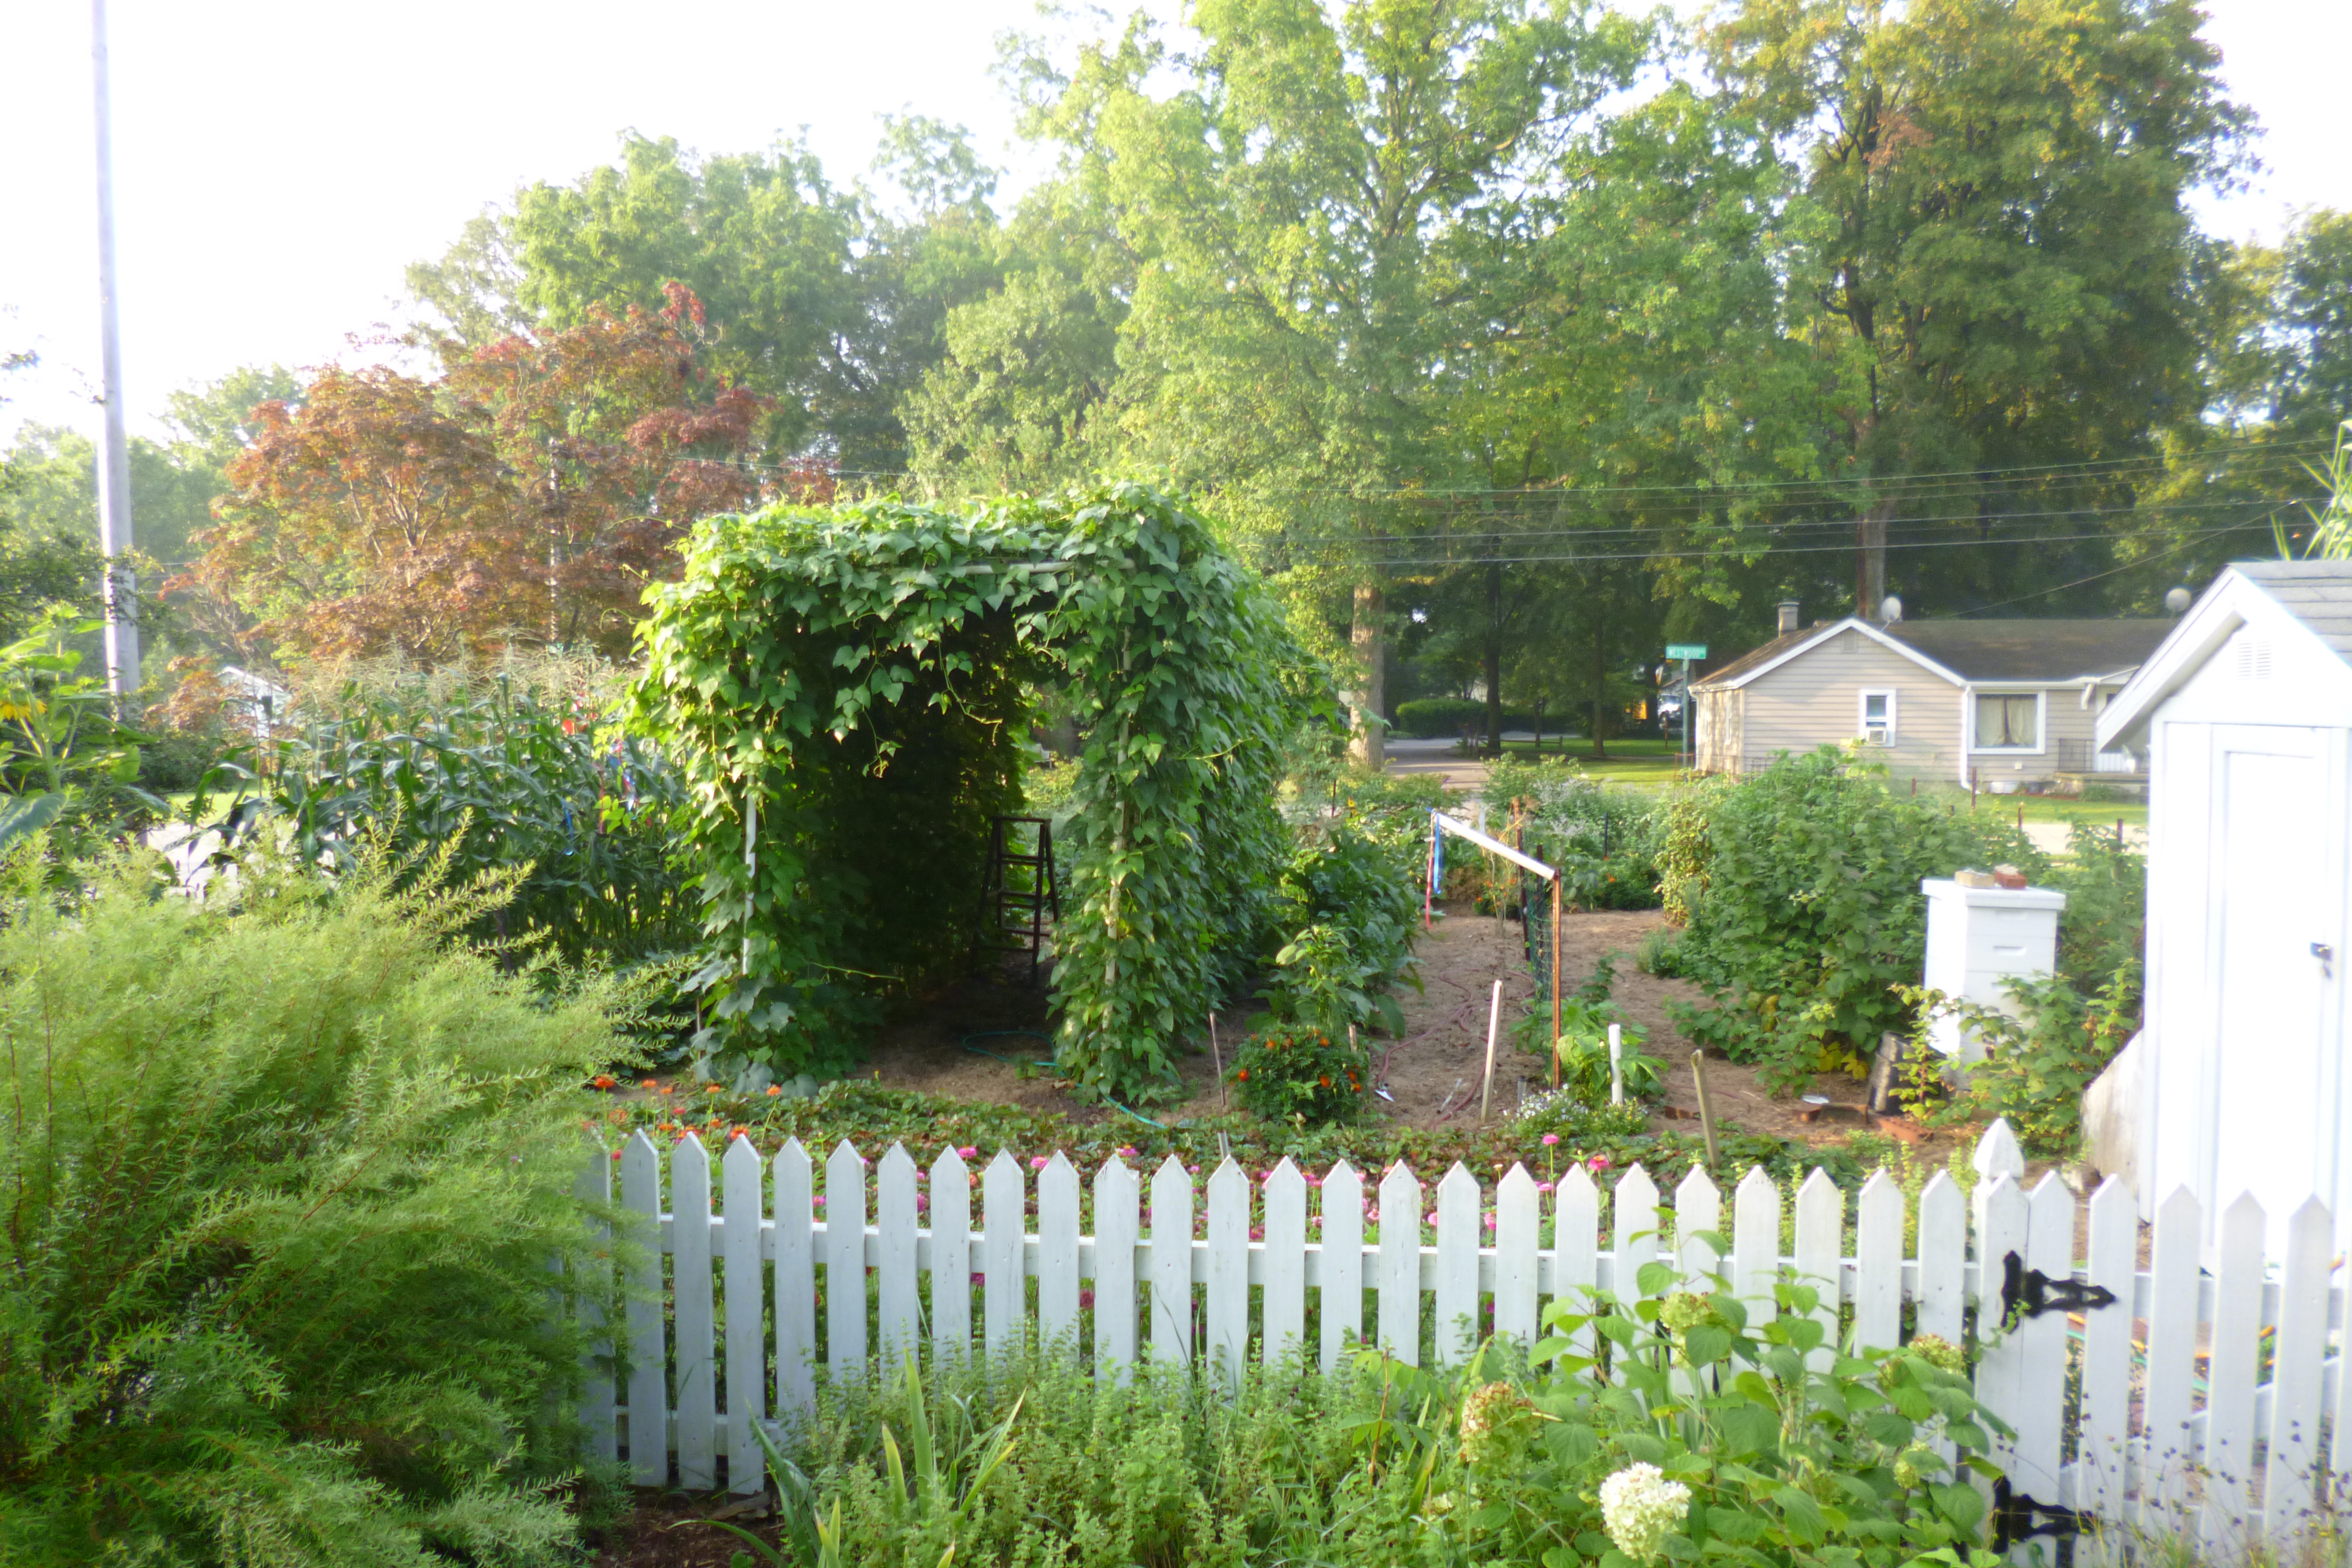
\includegraphics[width=0.9\textwidth]{our_family/16.jpg}
\caption{
"I CAN walk."
}
\end{figure}
In school he had no problem learning except when the subject did not interest him.
He excelled at playing chess and there is a box of trophies in the basement to prove it.

He was interested in the way things fit together and how they worked.
\begin{figure}
\centering
\includegraphics[width=0.9\textwidth]{our_family/17.jpg}
\caption{
"What does the world look like upside down?"
}
\end{figure}

From Abby - What a fun set of memories and descriptions.
I am so glad to have you as a mother and to have Tim and Jonathan as brothers.





